\label{chap:4}
\section{Simulação}\label{sec:simulation}

Simulamos a resposta ao impulso de uma sala utilizando o algoritmo Image-Source Model \cite{simulation}.

A sala utilizada nas simulações tem dimensões $4,45m \times 3,55m \times 2,5m$ (largura × comprimento × altura) e é completamente selada. Além disso, o coeficiente de absorção de todas as suas paredes é o mesmo, considerando que todas são feitas do mesmo material. O material utilizado altera o tempo de reverberação, sendo que o algoritmo de simulação calcula o coeficiente de absorção das paredes da sala dependendo do tempo de reverberação escolhido. O arranjo de microfones é linear e foi posicionado em torno do ponto $Mic_c$ = [2 1,5 1,6]$^T$. Foi simulado apenas o cenário com 2 microfones e 2 fontes. Os sinais das fontes têm $10s$ de duração, consistindo em sinais de voz masculino e feminino e foram distribuídas em torno do centro do arranjo, com dois parâmetros para identificá-las: o DOA de cada uma, e a distância delas até o arranjo. O tempo de reverberação utilizado nesta dissertação é o ${T_{60}}$, que é o tempo requerido para que a energia das componentes relativas a reflexões do sinal caia a 60 dB abaixo do nível do som direto. A janela utilizada para a STFT é a janela de \textit{Hanning} de comprimento $L$ igual à $4096$ pontos.

As fontes utilizadas foram do SASSEC, correspondendo a dois trechos de sinais de voz de 10 segundos de duração cada, amostrados a 16 kHz. Um sinal é composto de uma voz masculina, enquanto o outro é composto por uma voz feminina. Decimamos os sinais para que a frequência de amostragem fosse reduzida para 8 kHz. As informações do ambiente simulado são dadas na Figura \ref{fig:environment}.

\begin{figure}
    \centering
    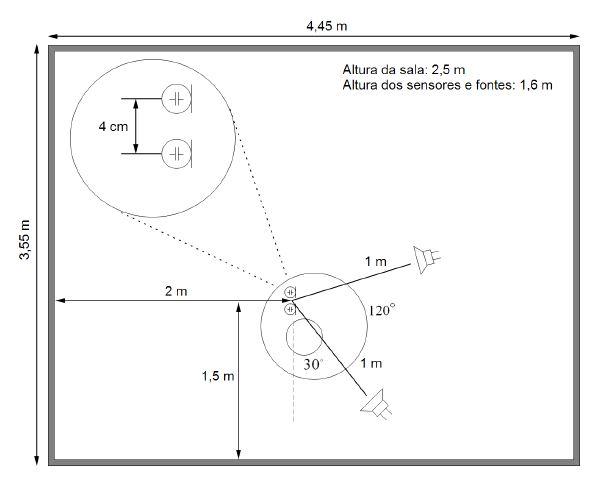
\includegraphics{environment.JPG}
    \caption{Configuração da sala utilizada nos testes. Todas as cotas da figura estão dadas em metros. A sala possui as dimensões $4,45m \times 3,55m \times 2,5m$ (comprimento, largura e altura). Todo o ambiente é selado, i.e., não há portas ou janelas. Os microfones (sensores) encontram-se separados por uma distância de $4cm$ e o centro deste arranjo é representado pelo vetor $Mic_c$ = [2 1,5 1,6]$^T$. As fontes 1 e 2 estão à distância de $1m$ do centro do arranjo de microfones e estão dispostas a $\frac{2\pi}{3}$ e $\frac{\pi}{6}$ em relação à ordenada, respectivamente.}
    \label{fig:environment}
\end{figure}


 \section{Análise dos Algoritmos}\label{sec:analysis}
    
    Nas condições de simulação descritas na Seção \ref{sec:simulation}, comparamos os métodos ICA-EBM e Natural ICA em relação aos resultados e à performance quanto à separação dos sinais. Vale ressaltar que o objetivo destes experimentos foi avaliar unicamente a etapa de separação dos sinais e, por isso, não houve qualquer alteração no método de resolução da permutação e de escalonamento. 
    
    Inicialmente, a simulalação foi feita com tempo de reverberação $T_{60}$ igual a $0.1s$ e comprimento da janela $L=2048$. Neste cenário, os sinais das fontes e dos sensores são mostrados nas Figuras \ref{fig:sources} e \ref{fig:sensors}, respectivamente. Após aplicar a STFT (definida na Seção \ref{sec:stft}) para transformar os sinais para o domínio da frequência e fazer a separação das fontes, incluindo tanto a etapa de pré-processamento (descrita na Seção \ref{sec:whitening}) quanto a de pós-processamento (apresentada na Seção \ref{sec:tdoa}), obtivemos as estimativas das fontes mostradas nas Figuras \ref{fig:icaebm} e \ref{fig:natica} para os métodos ICA-EBM e Natural ICA, respectivamente. Para este caso, ambos os métodos geraram boas estimativas das fontes, além de apresentarem desempenho similar.
    
    Posteriormente, aumentou-se o tempo de reverberação $T_{60}$ do ambiente de simulação, mantendo-se o comprimento da janela $L=2048$. Os tempos de reverberação utilizados nas simulações foram de $0.1s$, $0.25s$, $0.5s$ e $0.75s$. Nas Figuras \ref{fig:reverb_estimative_src_1} e \ref{fig:reverb_estimative_src_2} é mostrada uma comparação de desempenho entre os algoritmos usando as métricas descritas na Seção \ref{metrics} (em dB) para as estimativas das fontes 1 e 2, respectivamente. A Figura \ref{fig:comparison_convergence_ts} mostra o tempo de processamento (em segundos) para cada escolha do tempo de reverberação $T_{60}$ de ambos os algoritmos. Devido à queda no valor destas métricas com o aumento do tempo de reverberação $T_{60}$, é possível concluir que ambos os algoritmos passaram a ter suas estimativas degradadas. Além disso, apesar do desempenho ligeiramente superior do algoritmo ICA-EBM para praticamente todos os tempos de reverberação $T_{60}$, o algoritmo Natural ICA + FastICA apresenta um tempo de processamento significantemente menor para todos os tempos de reverberação $T_{60}$.
    
    Por fim, fixou-se o tempo de reverberação $T_{60}=0.5s$ e variou-se o tamanho da janela $L$ para os valores $256$, $512$, $1024$ e $2048$. O efeito deste parâmetro sobre as métricas de desempenho da Seção \ref{metrics} (em dB) está representado nas Figuras \ref{fig:window_estimative_src_1} e \ref{fig:window_estimative_src_2} para as estimativas das fontes 1 e 2, respectivamente. A Figura \ref{fig:comparison_convergence_window} mostra o tempo de processamento (em segundos) dos algoritmos Natural ICA e ICA-EBM em função do comprimento da janela $L$. Para todos os comprimentos de janela $L$, é possível verificar que o tempo de processamento do algoritmo Natural ICA + FastICA é menor. Entretanto, o algoritmo ICA-EBM apresenta resultados melhores para praticamente todas as janelas com comprimentos $L$ maiores que $256$.
    
    \begin{figure}
        \centering
        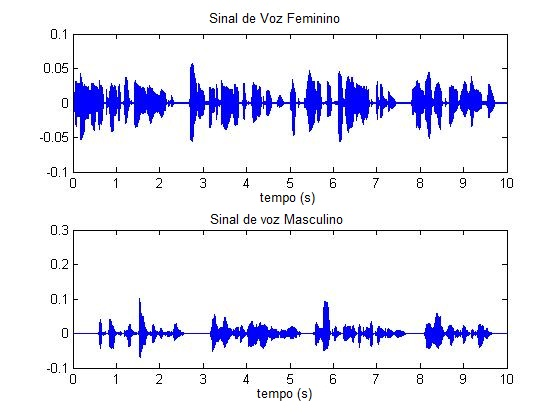
\includegraphics[scale=0.7]{sources.jpg}
            \caption{Sinais de cada uma das fontes no domínio do tempo.}
        \label{fig:sources}
        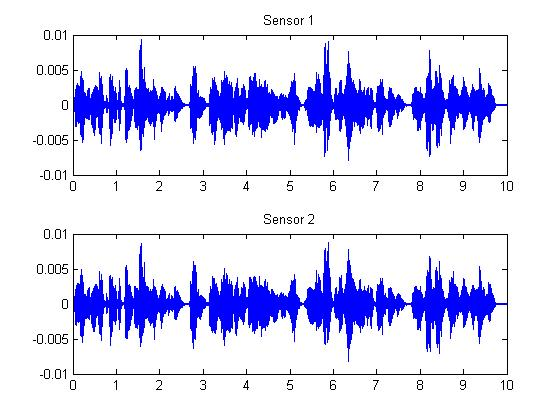
\includegraphics[scale=0.7]{sensors.jpg}
            \caption{Sinais em cada um dos sensores no domínio do tempo para $T_{60} = 0.1s$.}
        \label{fig:sensors}
    \end{figure}
    
    \begin{figure}
        \centering
        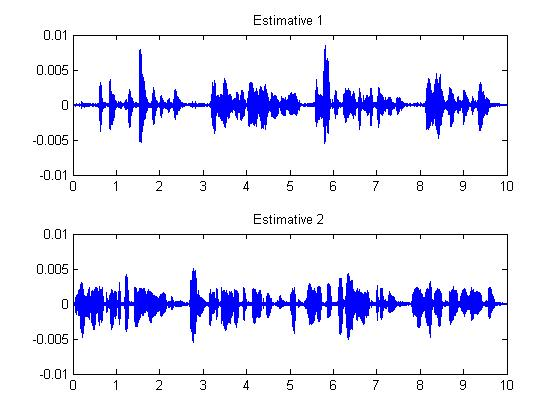
\includegraphics[scale=0.7]{estimatives_FASTICA.jpg}
            \caption{Sinais de estimativa das fontes obtidas pelo algoritmo ICA-EBM no domínio do tempo para $T_{60} = 0.1s$.}
        \label{fig:icaebm}
        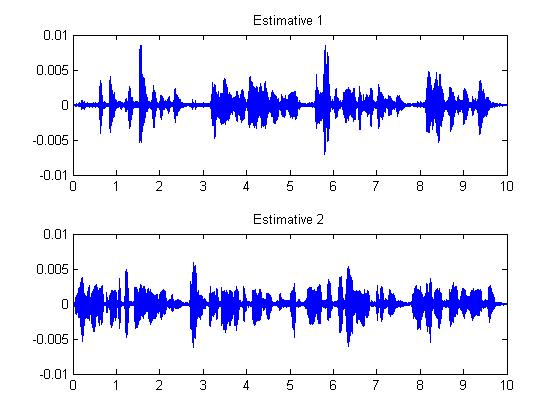
\includegraphics[scale=0.7]{estimatives_NATICA.jpg}
            \caption{Sinais de estimativa das fontes obtidas pelo algoritmo Natural ICA + FastICA  no domínio do tempo para $T_{60} = 0.1s$.}
        \label{fig:natica}
    \end{figure}
    
    \begin{figure}
        \centering
        \subfigure[Métricas de desempenho para a estimativa da fonte 1.]
        {
            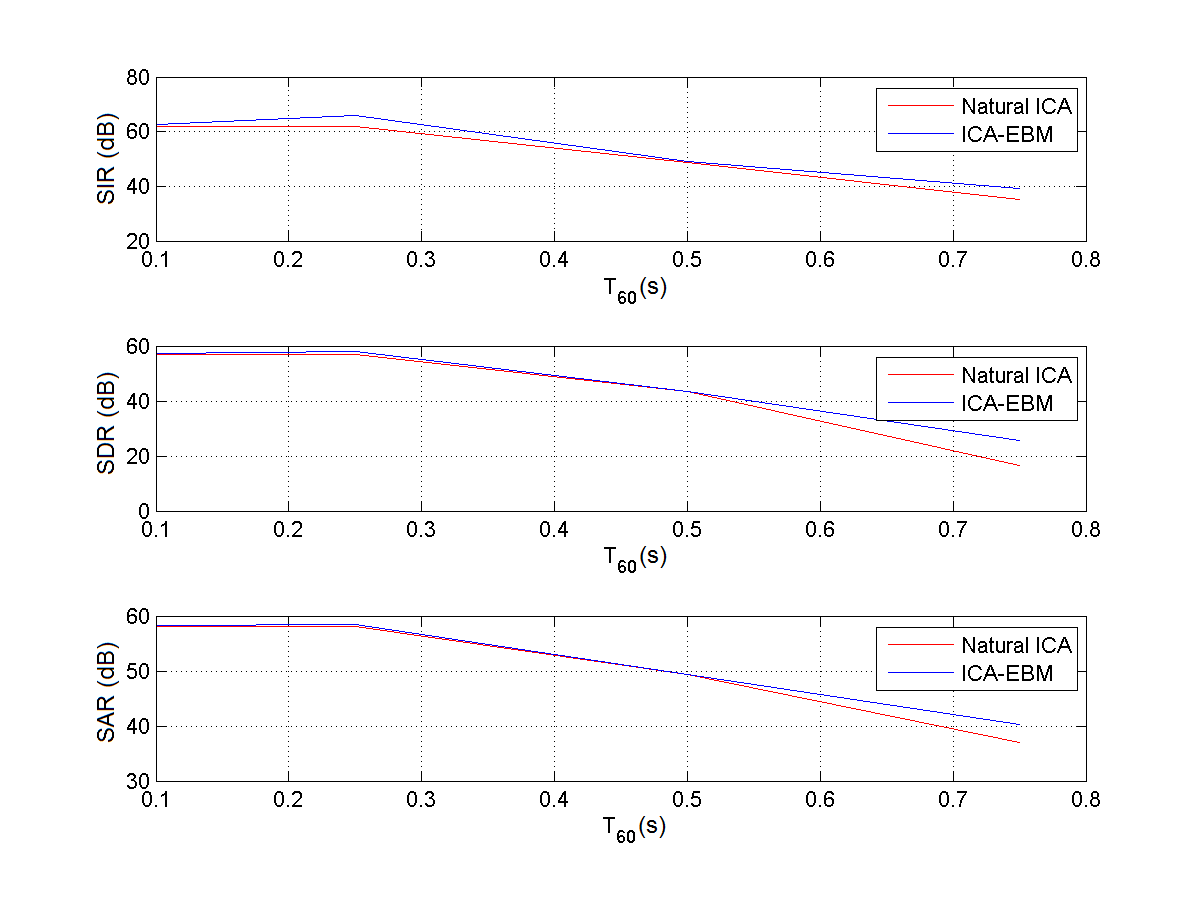
\includegraphics[scale=0.6]{figuras/reverb_estimative_src_1.png}
            \label{fig:reverb_estimative_src_1}
        }
        \\
        \subfigure[Métricas de desempenho para a estimativa da fonte 2.]
        {
            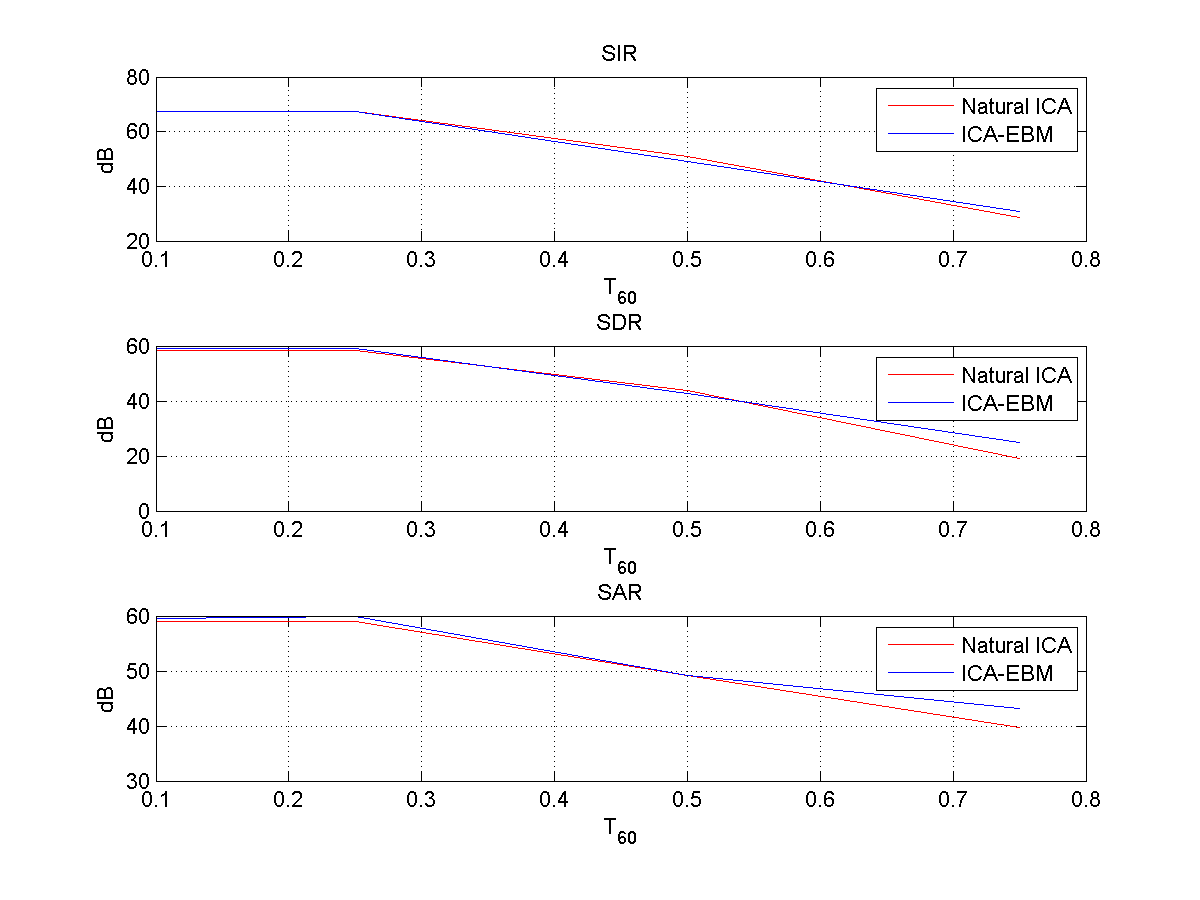
\includegraphics[scale=0.6]{figuras/reverb_estimative_src_2.png}
            \label{fig:reverb_estimative_src_2}
        }
        \caption{Métricas de desempenho dos algoritmos Natural ICA + FastICA e ICA-EBM (em dB) em função do tempo de reverberação $T_{60}$ (em segundos). É possível verificar a queda do desempenho em ambos os algoritmos através da evolução dos valores das métricas SIR, SDR e SAR     provocado pelo aumento do tempo de reverberação, além do desempenho ligeiramente     superiror do algoritmo ICA-EBM em relação ao Natural ICA + FastICA para praticamente     todos os tempos de reverberação.}
        \label{fig:reverb_estimative}
    \end{figure}

      
\begin{figure}
    \centering
        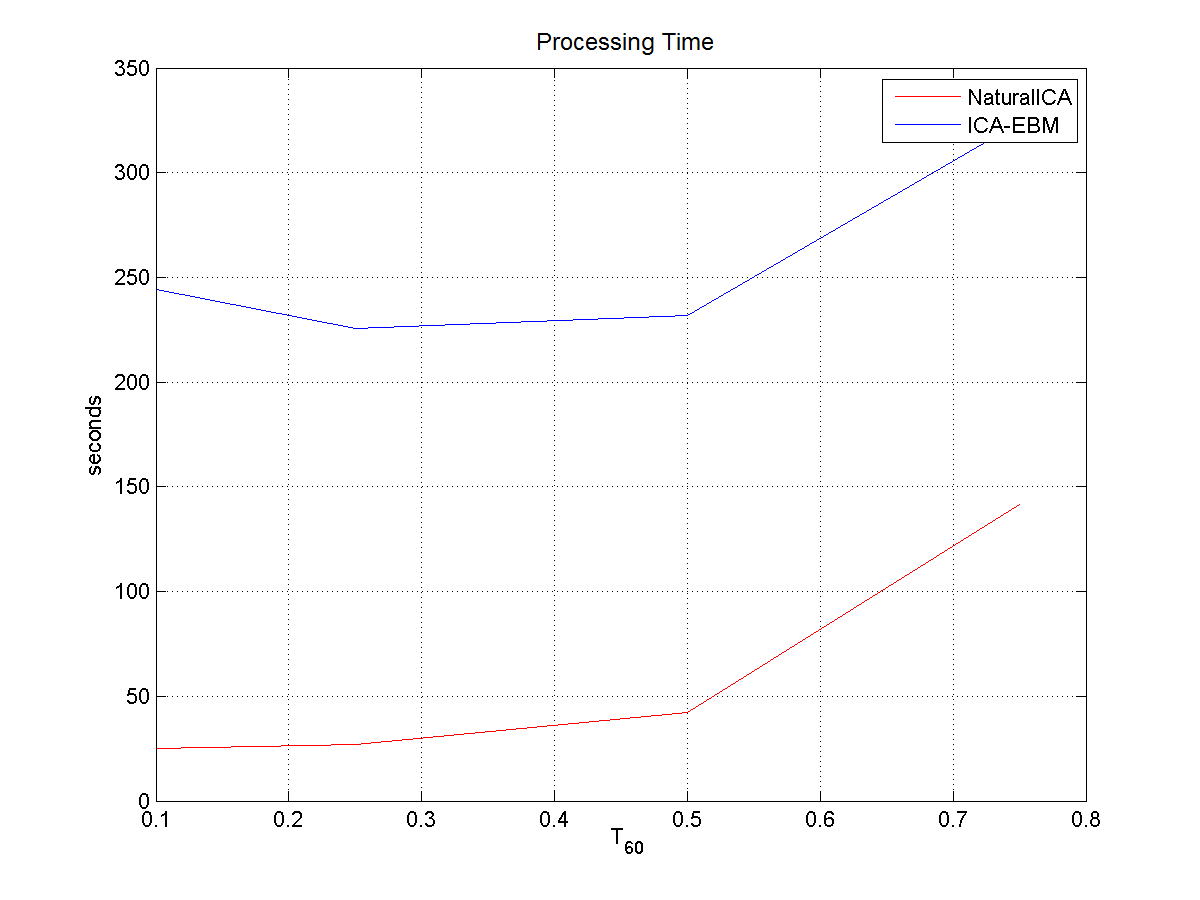
\includegraphics[scale=0.5]{figuras/comparison_convergence_ts.png}
            \caption{Tempo de processamento dos algoritmos ICA-EBM e Natural ICA + FastICA (em segundos) em função do tempo de reverberação do ambiente $T_{60}$ (em segundos). Ambos os algoritmos levam mais tempo para processar conforme o tempo de reverberação aumenta, mas o algoritmo Natural ICA + FastICA leva consideravelmente menos tempo do que o ICA-EBM para qualquer $T_{60}$.}
    \label{fig:comparison_convergence_ts}
\end{figure}


\begin{figure}
    \centering
    \subfigure[Métricas de desempenho para a estimativa da fonte 1.]
    {
        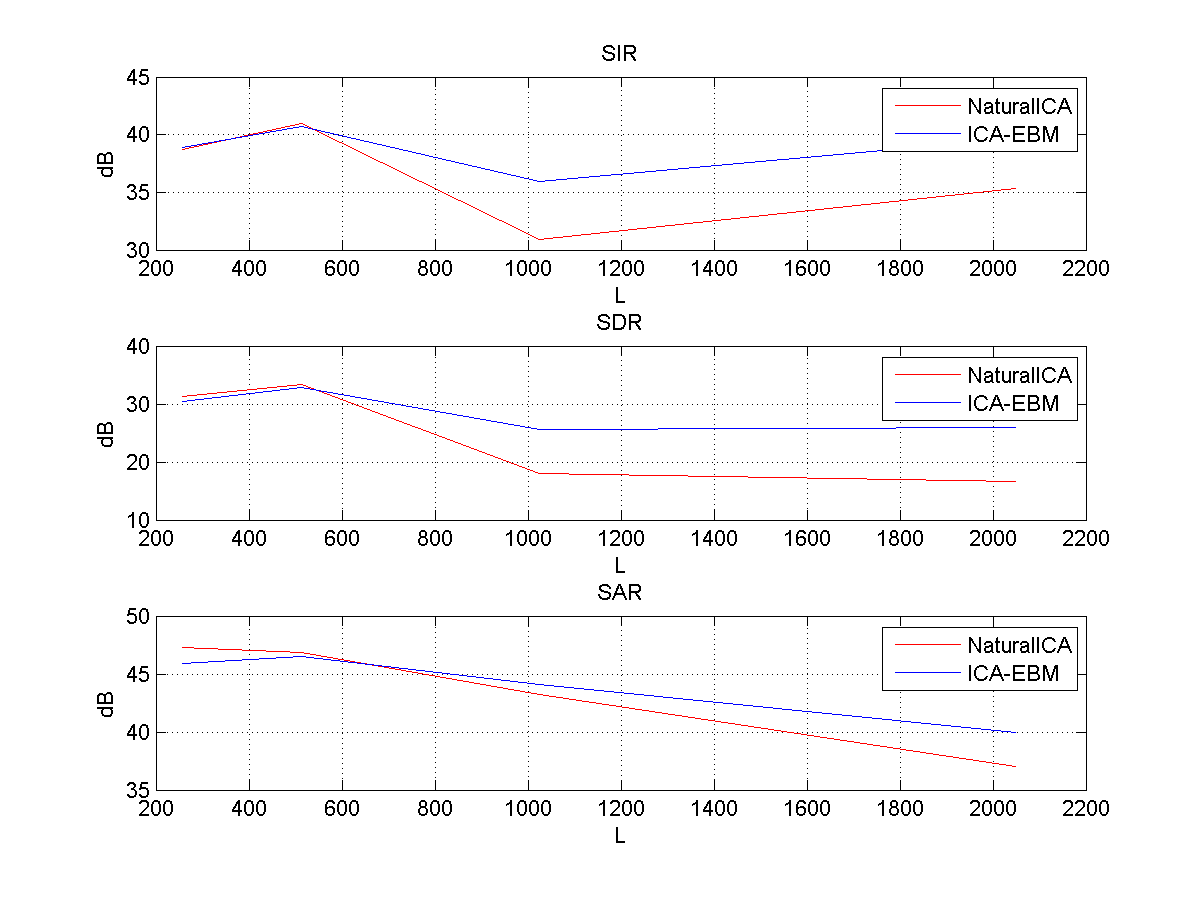
\includegraphics[scale=0.6]{figuras/window_estimative_src_1.png}
        \label{fig:window_estimative_src_1}
    }
    \\
    \subfigure[Métricas de desempenho para a estimativa da fonte 2.]
    {
        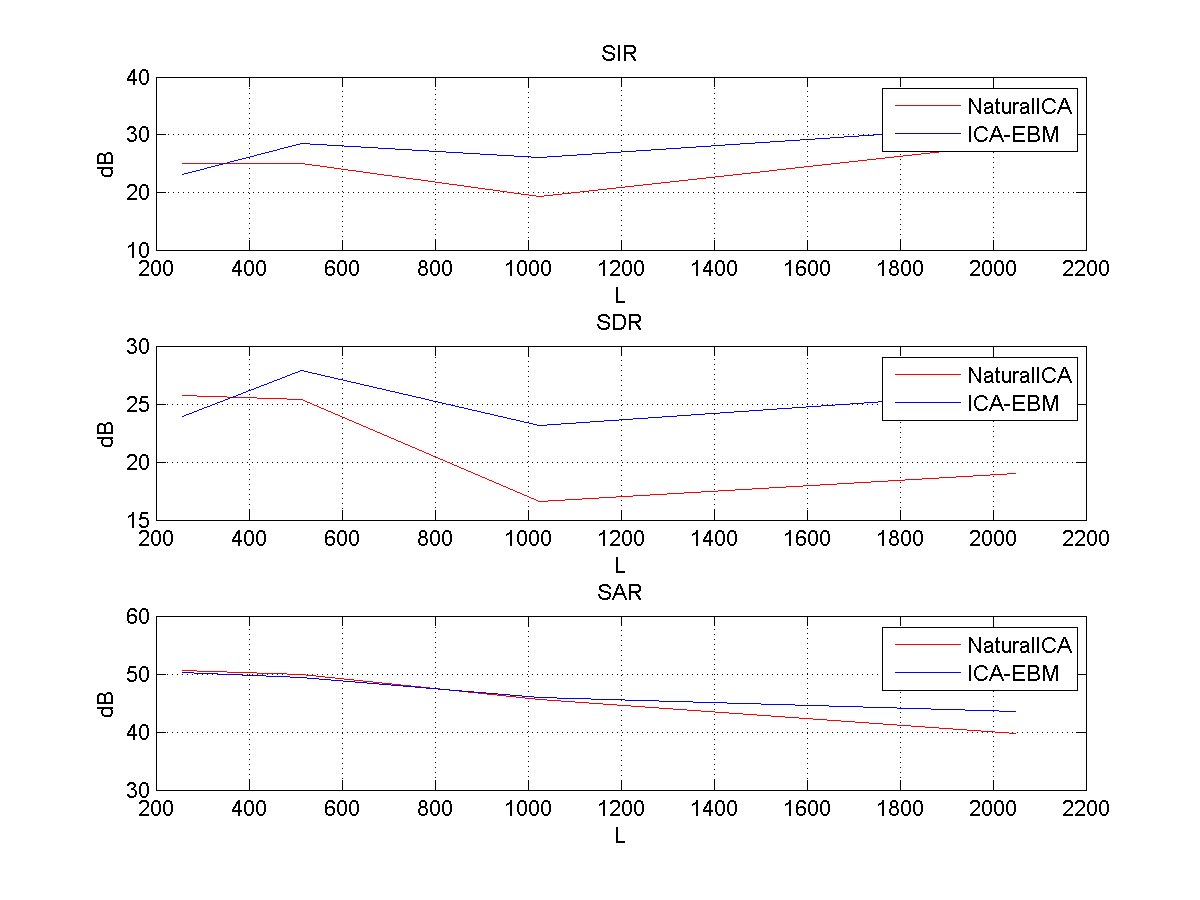
\includegraphics[scale=0.6]{figuras/window_estimative_src_2.png}
        \label{fig:window_estimative_src_2}
    }
    \caption{Métricas de desempenho dos algoritmos Natural ICA + FastICA e ICA-EBM (em dB) em função do comprimento da janela $L$ (em número de pontos). O algoritmo ICA-EBM apresenta um desempenho igual ou superior para todas as janelas com comprimento $L$ maior do que $256$.}
    \label{fig:window_estimative}
\end{figure}

\begin{figure}
    \centering
        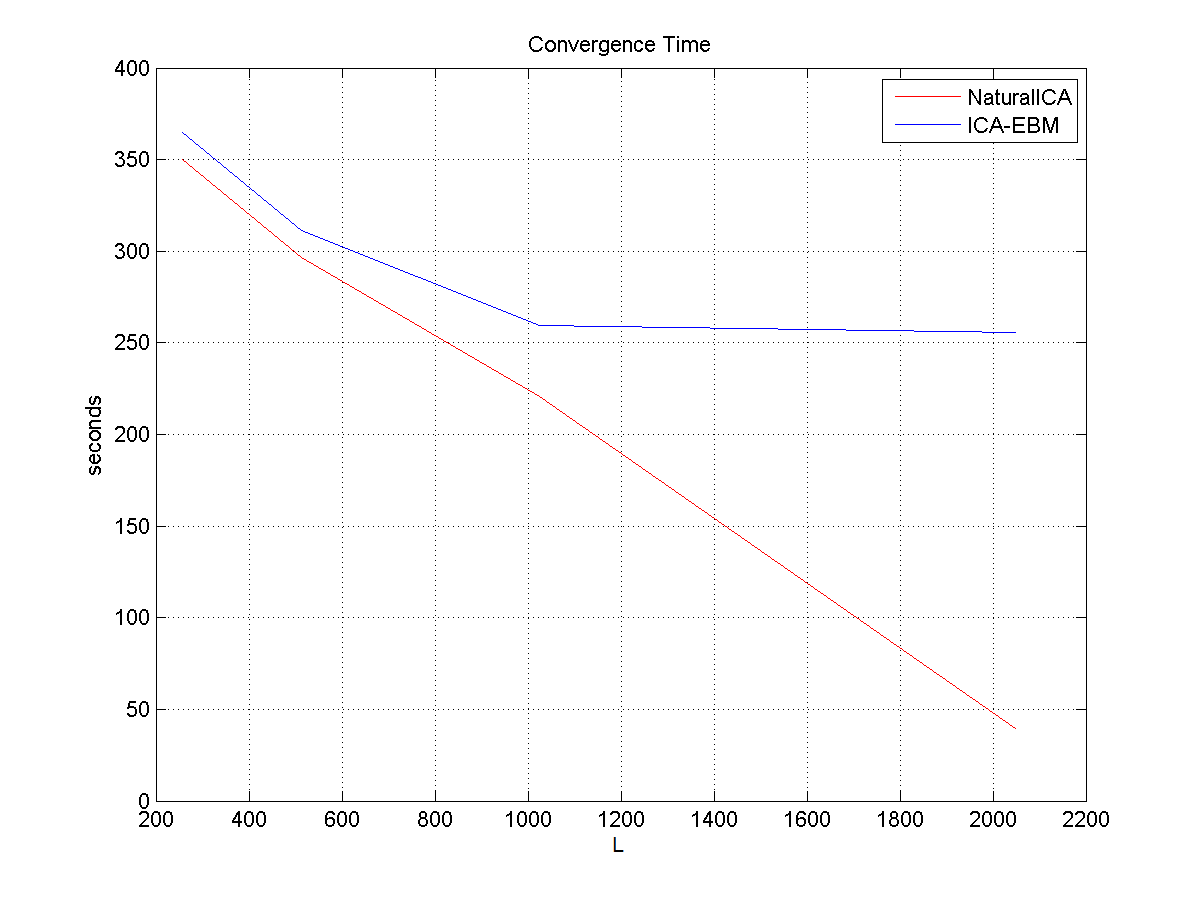
\includegraphics[scale=0.5]{figuras/comparison_convergence_window.png}
            \caption{Tempo de processamento dos algoritmos ICA-EBM e Natural ICA + FastICA (em segundos) em função do comprimento da janela $L$ (em número de pontos). Os algoritmos possuem tempos de processamento relativamente próximos até a janela de comprimento $L=1024$. Para comprimentos maiores, o algoritmo Natural ICA + FastICA passa a ter uma queda bem mais acentuada no seu tempo de processamento em relação ao ICA-EBM.}
    \label{fig:comparison_convergence_window}
\end{figure}
